\chapter{Detalii de implementare}

Scopul extensiei create este de prelua un fișier PDF încărcat de profesor într-un formular din Moodle și de a genera automat module de învățare și teste grilă, teste cu patru variante de
răspuns și doar una corectă, pe baza informațiilor din fișier. Mediul de dezvoltare folosit este XAMPP, cu un server Apache, limbajul de programare PHP, o bază de date MariaDB, și
platforma Moodle instalată local. Generarea conținutului educațional pe baza materialului încărcat se face cu ajutorul API-ului Gemini de la Google, care oferă un model de inteligență 
artificială capabil să extragă și să reformuleze text pentru a genera module de învățare și să creeze întrebări cu un singur răspuns corect pentru testele ce faciliteaza trecerea individului 
la următorul nivel.  

\section{Arhitectura generală}

Arhitectura sistemului utilizează modelul client-server. Clientul este reprezentat de interfața Moodle, iar aceasta diferă în funcție de rolul utilizatorului. Pentru profesor, extensia va 
fi vizibilă sub forma unei activități Moodle și va putea fi adăugata ca orice altă activitate, cum ar fi Quiz, Lecție sau orice altă activitate preinstalată de configurația standard. 
După selectarea extensiei, profesorul va avea parte de un formular unde poate încărca documentul în format PDF, iar extensia va crea automat modulele în urma completării acesteia. 
După generarea modulelor profesorul selectează dacă le salvează sau le generează încă o dată. În urma salvării acestora, profesorul le poate vizualiza și este informat de progresul studenților 
ce au inceput această activitate, printr-un tabel unde este trecut numele studentului, modulul la care se află și ora la care a început modulul. Pentru student, interfața permite începerea
activității, unde studentul susține un test pentru a de la ce modul este asignat pentru a-și începe studiul, vizualizarea modulului de învățare curent și a testului generat pe baza căruia 
îi este facilitată trecerea la următorul modul. Serverul este aplicația Moodle încărcată local pe care este instalată extensia. Backend-ul extensiei se ocupă cu preluarea 
fișierului PDF, gestionarea permisiunilor de acces, încărcarea informațiilor în baza de date și comunicarea cu API-ul Gemini, folosit pentru generearea conținutului din cadrul modulelor și 
a testelor.

\begin{figure}[ht]
    \centering
    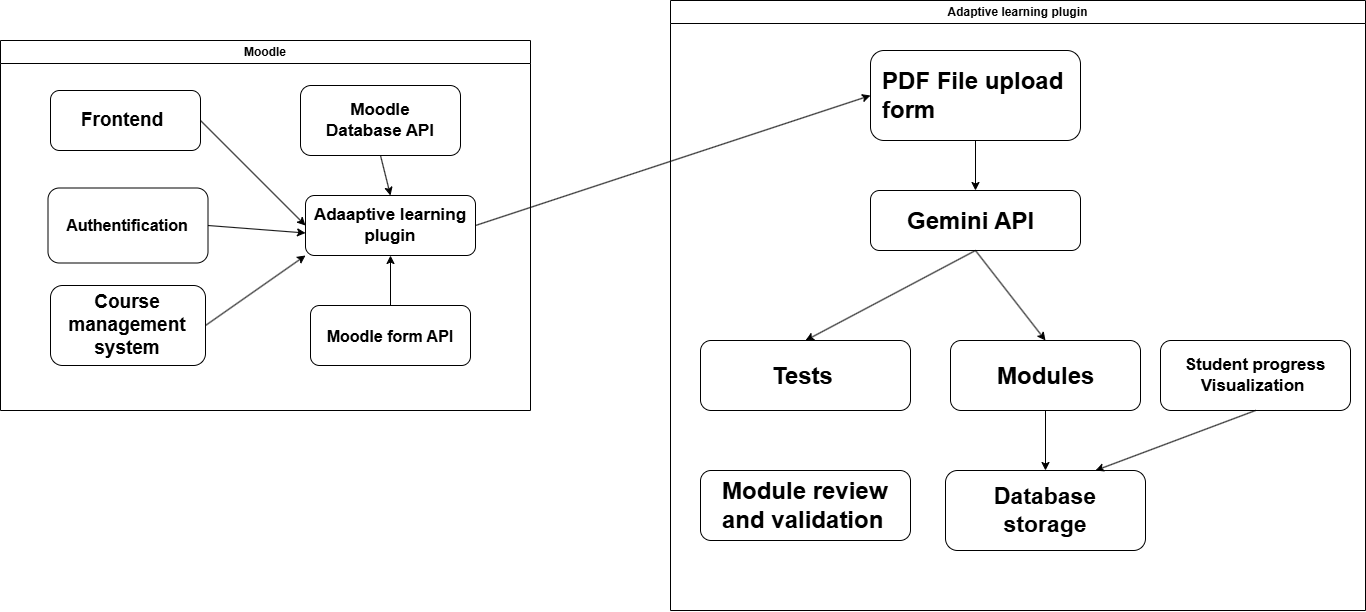
\includegraphics[width=0.8\textwidth]{images/LicentaArchitectureDiagram.png}
    \caption{Arhitectura generală a extensiei}
    \label{fig:arch_diagram}
\end{figure}

\section{Structura generală a extensiei Moodle}

Extensia dezvoltată este un plugin de tip \textit{activity} pentru Moodle, parte a categoriei \textit{mod}. Conform standardelor Moodle de dezvoltare a extensiilor, fiecare modul de activitate 
trebuie să se regăsească în directorul \textit{/mod/} și respecte convenția de denumire \textit{mod\_[modname]}, în cazul acesta denumindu-se \textit{mod\_adaptivelearning}.[15] Toate extensiile 
moodle sunt structurate într-un mod specific, având un set de fișiere și directoare necesare pentru a putea fi detectate de Moodle și pentru a funcționa corect. 

\subsection{Fișierul \textit{version.php}}
Primul fișier este 
\textit{version.php}, fișier ce conține metadate despre extensie. Acest fișier este esențial pentru ca Moodle să recunoască extensia, să o instaleze și să o actualizeze. Acesta conține 
informații precum versiunea extensiei, versiunea Moodle necesară pentru a rula extensia, numele și descrierea acesteia, maturitatea și o listă de dependențe de alte extensiei.[14] 

\subsection{Directoarele \textit{lang/en}}
Directoarele 
\textit{lang/en} sunt fișiere de limbă în care trebuie să existe un fișier \textit{adaptivelearning.php} ce conține toate stringurile necesare pentru a traduce extensia în limba engleză. 
Aceste stringuri sunt folosite pentru a afișa text în interfața utilizatorului, iar ele sunt accesate prin API-ul \textit{get\_string()} al Moodle, ce primește ca parametri un identificator
string și componenta unde se regăsește și returnează textul corespunzător din fișierul de limbă.[14]

\subsection{Fișierul \textit{lib.php}}
Fișierul \textit{lib.php} acționeaza ca un punct de legătură între Moodle și extensia noastră. Acesta conține funcțiile pentru a integra extensia în Moodle, cum ar fi funcțiile de adăugare, 
acutalizare și ștergere a unei instanțe a extensiei, în cazul nostru a unei activități de tip \textit{adaptivelearning}. În același timp, în fișier se regăsesc și funcțiile folosite 
în cadrul altor fișiere, de exemplu metodele create pentru comunicarea cu Gemini API și cele de parsare a răspunsurilor primite.[14]

\subsection{Directorul \textit{db}}
Directorul \textit{db} conține fișierele necesare pentru a crea tabelele din baza de date, ce sunt folosite pentru a stoca informațiile generate de extensie. Fișierul \textit{install.xml}
este folosit pentru a defini structura tabelelor, cum ar fi numele coloanelor, tipurile de date și relațiile dintre tabele. Acest fișier este folosit de Moodle pentru a crea tabelele
în baza de date la instalarea extensiei. Fișierul \textit{upgrade.php} conține pașii de actualizare a bazei de date și include schema nouă a tabelelor, schimbările aduse setărilor și 
alte modificări realizate în timpul actualizării extensiei. Pentru a crea o reînoire, dezvoltatorul extensiei trebuie să folosească editorul \textit{XMLDB}, un editor vizual pentru
fișierele XML ale bazei de date, pentru a crea definițiile câmpurilor noi, să actualizeze fișierul \textit{install.xml}, să genereze fișierul \textit{upgrade.php} și să modifice numărul 
versiunii în fișierul \textit{version.php}. Ultimul fișier necesar din directorul \textit{db} este \textit{access.php}, ce definește permisiunile necesare pentru a accesa extensia. 
Acest fișier conține o listă de capabilități, fiecare cu un nume unic și o descriere, ce sunt folosite pentru a controla accesul la diferite funcționalități ale extensiei. Aceste capabilități
sunt apoi asociate cu rolurile din Moodle, cum ar fi profesor sau student, pentru a controla cine poate accesa extensia și ce acțiuni poate efectua.[14]

\section{Definirea tabelelor din baza de date}
Moodle utilizeaza un sistem independent de SGBD, XMLDB, pentru definirea tabelelor din baza de date. Acest sistem permite dezvoltatorilor să definească structura tabelelor, 
relațiile dintre acestea și să efectueze modificări fără a fi necesară scrierea manuală a interogărilor SQL. Fișierul \textit{db/install.xml} este folosit pentru a defini tabelele și 
câmpurile, cheile și comentariile necesare pentru extensie, iar Moodle generează automat interogările SQL necesare pentru a crea tabelele în baza de date. Tabelele definite sunt următoarele:
\begin{itemize}
    \item \textit{adaptivelearning}: Acest tabel stochează instanțele activității.
    \item \textit{adaptivelearning\_modules}: Acest tabel stochează modulele generate din fișierul PDF încărcat de profesor.
    \item \textit{adaptivelearning\_progress}: Acest tabel stochează progresul studenților în cadrul activității.
\end{itemize} 

Tabelul \textit{adaptivelearning} are rolul de a stoca informațiile despre activitatea creată de profesor în cadrul unui curs Moodle și conține următoarele câmpuri: \textit{id}, 
\textit{course}, \textit{name}, \textit{description}, \textit{createdby}, \textit{timecreated}. Câmpul \textit{id} este de tip \textit{int} și este cheia primară, autoincrementată,  a tabelului. 
Câmpul \textit{course} este de tip \textit{int} și reprezintă ID-ul cursului în cadrul căruia este creată activitatea, legând activitatea de tabelul \textit{course} din Moodle. Câmpul 
\textit{name} este de tip \textit{char(255)} și reprezintă numele activității, iar câmpul \textit{description} este de tip \textit{text} și reprezintă descrierea generală a activității. 
Câmpul \textit{createdby} este de tip \textit{int} și reprezintă ID-ul utilizatorului care a creat activitatea. Câmpul \textit{timecreated} este de tip \textit{int} și reprezintă timpul 
la care a fost creată activitatea, stocat în format Unix timestamp.

Tabelul \textit{adaptivelearning\_modules} are rolul de a stoca modulele de învățare generate de API-ul Gemini pe baza fișierului PDF încărcat de profesor și conține următoare\-le câmpuri:
\textit{id}, \textit{activityid}, \textit{moduleindex}, \textit{title}, \textit{content}, \textit{timecreated}. Câmpul \textit{id} este cheia primară, autoincrementată, a tabelului. Câmpul 
\textit{activityid} este de tip \textit{int} și reprezintă ID-ul activității la care este asociat modulul, legându-se de tabelul \textit{adaptivelearning}. Câmpul \textit{moduleindex}
este de tip \textit{int} și reprezintă indexul modulului în cadrul activității, pentru a păstra ordinea modulelor. Câmpul \textit{title} este de tip \textit{char(255)} și reprezintă titlul
modului, iar câmpul \textit{content} este de tip \textit{text} și reprezintă conținutul modulului generat de Gemini API. Câmpul \textit{timecreated} este de tip \textit{int} și reprezintă 
timpul la care a fost creat modulul.

Tabelul \textit{adaptivelearning\_progress} are rolul de a stoca progresul studenților în cadrul activității și conține următoarele câmpuri: \textit{id}, \textit{userid}, \textit{moduleid}, 
\textit{status}, \textit{attemptedat}. Câmpul \textit{id} este cheia primară, autoincrementată, a tabelului. Câmpul \textit{userid} este de tip \textit{int} și reprezintă ID-ul 
utilizatorului care a început activitatea, legându-se de tabelul \textit{user} din Moodle. Câmpul \textit{moduleid} este de tip \textit{int} și reprezintă ID-ul modulului la care se află 
studentul în cadrul activității, legându-se de tabelul \textit{adaptivelearning\_modules}. Câmpul \textit{status} este de tip \textit{char(50)} și reprezintă starea progresului studentului. 
Acest câmp poate avea două valori posibile: \textit{inprogress}, pentru modulul actual la care se află studentul și urmează să dea test pentru a înregistra progres, sau \textit{completed}, 
pentru modulele pe care studentul le-a finalizat prin susținerea și promovarea testului. Câmpul \textit{attemptedat} este de tip \textit{int} și reprezintă timpul la care studentul a început 
modulul.

Am ales această structură a tabelelor pentru a permite stocarea eficientă a informa\-ți\-i\-lor despre activitățile create de profesori, modulele generate și progresul studenților. Am separat 
responsabilitățile fiecărui tabel pentru a permite o gestionare mai ușoară a datelor și pentru a facilita interogările ulterioare și le-am legat între ele prin chei externe pentru a
asigura integritatea datelor. Această structură permite extensibilitate, astfel încât se pot adăuga noi funcționalități și tabele în viitor fără a afecta funcționarea actuală a extensiei.
Totodată, în cadrul tabelului \textit{adaptivelearning\_progress} am implementat o coloană \textit{status}, cu cele două valori posibile, și nu am stocat doar modulele la care studentul se
află în prezent, ci și cele pe care le-a finalizat pentru a putea implementa o pagină dedicată studentului, unde poate accesa toate modulele disponibile, iar această implementare necesită 
un număr mai redus de interogări.
\section{Paginile principale ale extensiei}

\subsection{Pagina \textit{mod\_form.php}}

Prima pagina din cadrul extensiei este cea a formularului de configurare a activității \textit{mod\_form.php}, la care are acces doar profesorul pentru a adăuga o instanță de tip \textit{adaptivelearning} în cadrul unui curs 
Moodle. Această pagină este accesibilă din meniul de adăugare a activităților și resurselor, iar profesorul poate completa numele activității, descrierea acesteia și poate încărca un fișier 
PDF pe care dorește să îl folosească ca sursă de informații pentru generarea modulelor de învățare de către Gemini API. Formularul a fost creat folosind clasa \textit{moodleform}, 
ce oferă funcționalități pentru a crea formulare în Moodle. În urma salvării formularului, va fi apelată funcția \textit{add\_instance()} din fișierul \textit{lib.php}, care va crea o 
instanță a activității în baza de date și va salva informațiile completate de profesor. După apelul acestei funcții, extensia va redirecționa profesorul la pagina \textit{view.php}. 
Într-o extensie Moodle completarea formularului din interfață este direct legată de funcția \textit{add\_instance()} din fișierul \textit{lib.php}, care este responsabilă de crearea unei 
instanțe a activității, datorită mecanismului intern al Moodle. După salvarea formularului, Moodle valideaza datele introduse, creează un obiect \textit{\$data} cu valorile trimise și apelează 
funcția \textit{add\_instance()}, cu parametrii \textit{\$data} și \textit{\$mform}, din \textit{lib.php}, funcție ce inserează înregistrarea activității în tabelul \textit{adaptivelearning}. 
Pentru salvarea fișierului PDF încărcat de profesor, extensia folosește funcția \textit{file\_save\_draft\_area\_files()} din Moodle și apelează funcția 
\textit{adaptivelearning\_generate\_modules\_from\_pdf()}, funcție creată, responsabilă cu preluarea fișierului și comunicarea cu Gemini API pentru generarea modulelor de învățare. În urma 
adăugă\-rii instanței, extensia va redirecționa profesorul la pagina \textit{view.php}.[17]

\subsection{Pagina \textit{view.php}}
Pagina \textit{view.php} este pagina principală a activității, unde profesorul poate vizualiza informațiile despre activitate, modulele generate și progresul studenților. Înainte de afișarea 
conținutului paginii, extensia verifică dacă modulele activității există în baza de date, iar dacă nu există, va redirecționa utilizatorul la pagina de \textit{review.php} unde profesorul 
salvează modulele generate. Totodată, extensia verifică dacă utilizatorul are permisiunea de a accesa pagina, verificând dacă acesta are permisiunea de a adăuga o instanță. Dacă utilizatorul 
nu are permisiunea de a adăuga o instanță, înseamnă că este student, iar acesta va fi redirecționat la pagina \textit{learn.php} cu ajutorul funcției \textit{redirect()}. Pagina fiind 
destinată doar profesorilor, va afea afișate toate modulele, titlul și conținutul acestora, folosind funcția \textit{get\_records()} din Moodle, ce are ca parametrii numele tabelului și
condițiile de filtrare și returnează toate înregistrările din tabel. În cazul de față am selectat toate înregistrările din tabelul \textit{adaptivelearning\_modules} unde câmpul 
\textit{activityid} este egal cu ID-ul activității curente. Totodată, extensia va afișa și progresul studenților în cadrul activității, folosind funcția \textit{get\_records\_sql()} din 
Moodle, funcție ce permite executarea interogărilor SQL personalizate și returnează rezultatele sub formă de obiecte. Am ales această funcție deoarece aveam nevoie de o interogare SQL în 
care să dau join între tabelele \textit{adaptivelearning\_progress} și \textit{user} pentru a identifica utilizatorilor și între tabelele \textit{adaptivelearning\_modules} și
\textit{adaptivelearning\_progress} pentru a identifica modulele la care se află fiecare student. În tabelul rezultat vor fi afișate numele studentului, prin funcția \textit{fullname()} 
din Moodle care primește ca parametru un obiect de tip \textit{user}, titlul modulului curent, și ora la care studentul a început modulul. Vor fi afișați doar studenții care au un modul cu 
statusul \textit{inprogress} asupra unui modul din cadrul activității curente, pentru a nu afișa studenții care au finalizat toate modulele. În cazul în care nu există studenți care să fi 
început activitatea sau toți studenții care au început activitatea deja au terminat-o,  extensia va afișa un mesaj corespunzător folosind funcția Moodle \textit{notification()}.

\subsection{Pagina \textit{review.php}}
Pagina \textit{review.php} este pagina unde profesorul poate vizualiza modulele generate de Gemini API și poate decide dacă le salvează sau le generează încă o dată. Această pagină este
accesibilă doar profesorului, prin redirecționare de la pagina \textit{view.php} după completarea formularului, formular la care doar profesorul are acces. Răspunsul primit de la Gemini API 
este salvat în sesiune și este folosit pentru a afișa modulele generate în cadrul paginii. O sesiune este o stocare temporară pe server care reține date între mai multe cereri HTTP ale 
aceluiași utilizator. PHP creează automat un ID de sesiune care este trimis browserului sub forma unui cookie. Browserul trimite inapoi acest ID la fiecare cerere, iar PHP îl folosește 
pentru identificarea datelor salvate ale acelui utilizator. Profesorul are două butoane 
disponibile, \textit{Save} și \textit{Regenerate}. Dacă profesorul apasă butonul \textit{Save}, extensia va salva modulele în baza de date, folosind funcția \textit{insert\_record()}, ce 
are ca parametru un obiect de tip \textit{stdClass} cu atributele necesare pentru a crea o înregistrare în tabelul \textit{adaptivelearning\_modules}. Dacă profesorul apasă butonul 
\textit{Regenerate}, extensia va apela funcția \textit{adaptivelearning\_generate\_modules\_from\_pdf()} din fișierul \textit{lib.php}, care va trimite din nou fișierul PDF la Gemini API, 
iar întreg procesul de salvare a modulelor va fi repetat cu noile module generate.

\subsection{Pagina \textit{learn.php}}
Pagina \textit{learn.php} este pagina destinată studenților, unde aceștia pot începe activitatea de învățare. Această pagină este accesibilă doar studenților, iar această verificare este 
realizată în pagina \textit{view.php} prin verificarea permisiunilor de creare a unei instanțe a activității, iar doar cei ce nu au această permisiune vor fi redirecționați la 
\textit{learn.php}. În cadrul acestei pagini, studentul va vedea titlul și conținutul modulului curent, adică cel la care studentul are statusul \textit{inprogress} în tabelul 
\textit{adaptivelearning\_progress}. Înainte de a afișa conținutul modulului, extensia verifică dacă studentul are ultimul modul din cadrul activității cu statusul \textit{completed}, 
folosind funcția \textit{record\_exists\_sql()} din Moodle, funcție ce permite executarea interogărilor SQL și returnează un boolean în funcție de existența înregistrării. Interogarea SQL 
folosită realizează un join între tabelele \textit{adaptivelearning\_progress} și \textit{adaptivelearning\_modules}, verificând ID-ul activității curente, ID-ul studentului, statusul 
\textit{completed} și dacă modulul este ultimul din cadrul activității. Pentru a obține ID-ul ultimului modul din cadrul activității, realizez înainte o nouă interogare SQL prin intermediul 
funcției \textit{get\_field\_sql()}, funcție ce returnează valoarea unui câmp dintr-o interogare SQL. Această interogare selectează ID-ul modulului cu indexul maxim din tabelul
\textit{adaptivelearning\_modules} pentru activitatea curentă. Dacă ultimul modul are statusul \textit{completed}, studentul va fi redirecționat la pagina \textit{finish.php}, iar în 
cazul în care nu are ultimul modul completat, extensia va afișa conținutul modulului curent. Pentru a obține modulul curent, apelez funcția \textit{get\_record\_sql()} și folosesc o interogare SQL în care dau joint între tabelele 
\textit{adaptivelearning\_modules} și \textit{adaptivelearning\_progress} verificând ID-ul activității curente, ID-ul studentului și statusul \textit{inprogress}. Dacă studentul nu are 
niciun modul cu statusul \textit{inprogress}, acesta este redirecționat la pagina \textit{start.php}. Studentul are acces la două butoane, \textit{Take test} și \textit{See available modules}. 
Butonul \textit{Take test} redirecționează stundetul la pagina \textit{test.php}, unde va putea începe testul pentru a trece la următorul modul, iar butonul \textit{See available modules} 
redirecționează studentul la pagina \textit{available\_modules.php}, unde acesta poate vedea toate modulele disponibile din cadrul activității, adică toate modulele cu statusul
\textit{completed} sau \textit{inprogress}.

\subsection{Pagina \textit{start.php}}
Pagina \textit{start.php} este pagina de start a activității, unde studentul poate începe activitatea de învățare. Această pagină este accesibilă doar studenților, deoarece pentru a ajunge 
la ea, trebuie să fii redirecționat de la pagina \textit{learn.php}. Pagina conține o descriere a activităților de tip \textit{adaptivelearning} și un buton de start al activității.
După apăsarea butonului, studentul este redirecționat la pagina \textit{init\_test.php} și este creată o înregistrare în tabelul \textit{adaptivelearning\_progress}, folosind funcția 
\textit{insert\_record()}, cu statusul \textit{inprogress} pentru primul modul din cadrul activității.

\subsection{Pagina \textit{test.php} și \textit{init\_test.php}}
Paginile \textit{test.php} și \textit{init\_test.php} sunt implementate aproape identic deoarece pagina \textit{init\_test.php} folosește aceiași structură cu cea a paginii \textit{test.php}. 
Ambele pagini sunt accesibile doar studenților și afișează un test generat cu ajutorul funcției \textit{adaptivelearning\_generate\_quiz\_from\_module()} din fișierul \textit{lib.php}, 
funcție ce comunică cu Gemini API. Diferențele provin din rolul fiecărei pagini. Pagina \textit{init\_test.php} este folosită pentru a vedea la ce modul va fi distribuit studentul. Prima 
oară va primi un test pentru primul modul, iar dacă îl promovează va primi testul pentru următorul modul și va fi creată o înregistrare în tabelul \textit{adaptivelearning\_progress} 
cu statusul \textit{inprogress} pentru modulul următor, iar înregistrarea pentru modulul curent va fi actualizată cu statusul \textit{completed}. Dacă studentul nu promovează testul,
înregistrarea pentru modulul curent va rămâne cu statusul \textit{inprogress} și studentul este redirecționat la pagina \textit{learn.php}. Totodată, studentul are acces la butonul 
\textit{skip} care îl redirecționează la pagina \textit{learn.php} fără a mai edita înregistrarea deja creată în baza de date, iar verificarea răspunsurilor date se face în cadrul 
aceleiași pagini. Pagina \textit{test.php} este folosită pentru a afișa testul generat de Gemini API destinat promovării la următorul modul. Verificarea răspunsurilor se face prin 
redirecționarea la pagina \textit{results.php} după apăsarea butonului \textit{Submit answers}. O altă diferență între cele două pagini este modul în care testul afișat este considerată
promovat. În pagina \textit{init\_test.php}, pentru a putea trece la testul următorului modul studentul trebuie să obțină minim 75\% întrebări cu răspuns corect. Deoarece nu mereu testul 
generat are un număr de întrebări multiplu de 4, am implementat o funcție care calculează procentul de întrebări corecte și dacă acesta este mai mare sau egal cu 75\%, studentul
trece la următorul modul. Pentru a promova testele din pagina \textit{test.php}, studentul trebuie să obțină minim 50\% + 1 întrebări corecte. Ambele tipuri de teste sunt formulare HTML
care conțin întrebările și răspunsurile sunt amestecate prin intermediul metodei \textit{shuffle()} din PHP, iar pentru fiecare răspuns este creat un input de tip \textit{radio}.

\subsection{Pagina \textit{results.php}}
Pagina \textit{results.php} este pagina unde studentul poate vedea rezultatele testului de promovare la următorul modul. După ce studentul completează testul generat, formularul HTML trimite 
datele prin metoda POST către pagina \textit{results.php}. Pagina are acces și la răspunsul primit de la Gemini API, ce conține întrebările și răspunsurile corecte și verifică dacă răspunsul 
studentului este același cu cel corect oferit de API. Răspunsurile corecte sunt stocate într-un array construit pe baza răspunsului primit de la Gemini API pentru a putea fi comparate cu
răspunsurile studentului. În urma verificării răspunsurilor, extensia va calcula procentul de întrebări corecte și va afișa un mesaj, folosind funcția \textit{notification()} din Moodle, 
pentru a informa studentul dacă a promovat sau nu testul. Dacă studentul a promovat testul, extensia va actualiza înregistrarea din tabelul \textit{adaptivelearning\_progress} pentru modulul 
curent, setând statusul la \textit{completed} și va crea o nouă înregistrare cu statusul \textit{inprogress} pentru următorul modul. În ambele situații în care studentul fie a promovat, fie 
nu a promovat testul, extensia va redirecționa studentul la pagina \textit{learn.php} prin intermediul butonului \textit{Continue learning}.

\subsection{Pagina \textit{available\_modules.php}}
Pagina \textit{available\_modules.php} este pagina unde studentul poate vedea toate modulele disponibile din cadrul activității. Modulele disponibile sunt cele cu statusul
\textit{completed} sau \textit{inprogress}. Afișarea modulelor se face printr-o interogare SQL cu join între tabelele \textit{adaptivelearning\_modules} și 
\textit{adaptivelearning\_progress}, selectând ID-ul modulului, titlul, conținutul acestuia și statusul progresului studentului, verificând ID-ul activității curente, ID-ul studentului 
și statusul \textit{completed} sau \textit{inprogress}. Dacă studentul nu are niciun modul disponibil, extensia va afișa un mesaj folosind funcția \textit{notification()}.

\subsection{Pagina \textit{finish.php}}
Pagina \textit{finish.php} este pagina finală a activității, unde studentul este înștiințat că a finalizat toate modulele din cadrul activității. Pagina afișează un mesaj pentru student 
și un buton de redirecționare la pagina \textit{available\_modules.php} pentru a putea vedea toate modulele disponibile.

\section{Interacțiunea cu Gemini API}
Extensia utilizează Gemini API pentru două funcționalități: generarea modulelor de învățare pe baza fișierului PDF încărcat de profesor și generarea testelor grilă pentru fiecare modul. 
Pentru a putea utiliza Gemini API, extensia trebuie să aibă un token de autentificare, ce este obținut prin intermediul unui cont Google Cloud Platform.
\subsection{Generarea modulelor de învățare} 
Trimiterea fișierului PDF este realizată prin intermediul metodei \textit{adaptivelearning\_}\\\textit{generate\_modules\_from\_pdf()}, ce are ca parametru fișierul PDF încărcat în formularul de 
configurare a activității. Fișierul este citit din \textit{file storage} folosind funcția \textit{get\_file\_storage()} din Moodle, iar conținutul binar este codificat în Base64 pentru a 
fi trimis la Gemini API. În cadrul acestei funcții este contruit payload-ul JSON necesar pentru a trimite fișierul PDF în care este inclus și promptul de generare a modulelor de învățare.
Apoi se face apelul HTTP POST catre endpoint-ul Gemini API, folosind funcția \textit{file\_get\_conten}\\\textit{ts()}, ce trimite datele către Gemini API și returnează răspunsul primit. 
Răspunsul este apoi decodat din JSON și se apelează funcția de parsare a răspunsului pentru a extrage modulele de învățare generate. Promptul pentru generarea modulelor de învățare 
a evoluat pentru a obține rezultate mai bune și pentru a extrage informații relevante din fișierul PDF. Primul prompt a fost:
\begin{quote}
    \textit{Împarte acest fișier PDF în module de învățare.}
\end{quote}

Acest prompt a fost prea general și nu oferea suficiente informații despre modul în care ar trebui să fie structurate modulele. Chiar dacă a fost realizată o împărțire bună a modulelor, 
conținutul fiecărui modul era prea scurt și era sub forma unui cuprins a ce se regăsește în acesta.

Următorul prompt încercat a fost:
\begin{quote}
    \textit{Împarte acest fișier PDF în 3 module de învățare, fiecare modul va avea un titlu si un text care va explica fiecare lucru din acel modul.}
\end{quote}

Acest prompt a oferit rezultate mai bune deoarece cuprindea toate informațiile necesare, dar formularea utilizată nu era cea potrivită, deoarece răspunsul primit povestea fiecare informație 
în loc să fie structurată ca un modul de învățare.

Următorul prompt încercat a fost: 
\begin{quote}
    \textit{Împarte acest fișier PDF în 3 module de învățare, fiecare modul va avea un titlu si un text care va explica in detaliu fiecare lucru din acel modul. Textul fiecarui modul va fi formulat ca un profesor}
\end{quote}

Acest prompt a oferit rezultate foarte bune, deoarece a structurat modulele de învățare în mod corespunzător, fiecare modul având un titlu și un conținut detaliat, dar adăuga\-rea formulării
textului ca un profesor, a făcut ca răspunsul să fie formulat ca un dialog pe care profesorul îl are cu o clasă de elevi sau studenți.

Promptul final folosit pentru generarea modulelor de învățare este:
\begin{quote}
    \textit{Împarte acest fișier PDF în 3 module de învățare, fiecare modul va avea un titlu si un text care va explica in detaliu fiecare lucru din acel modul. Textul fiecarui modul va fi formulat cu un limbaj academic. Raspunsul va fi strutcurat astfel: *titlu modul1*modul text1*titlu modul2*modul text2... si fara new line.}
\end{quote}

Acest prompt oferă toate informațiile necesare pentru a obține modulele de învățare structurate corespunzător, fiecare modul având un titlu și un conținut detaliat, iar răspunsul este
structurat într-un mod ușor de procesat. Răspunsul primit de la Gemini API este un string ce conține modulele separate prin \textit{*}, acest răspuns fiind apoi procesat de funcția
\textit{adaptivelearning\_parse\_modules()}, ce împarte stringul în module și extrage titlul și conținutul fiecărui modul.
\subsection{Generarea testelor grilă}
Generarea testelor grilă se face prin intermediul funcției \textit{adaptivelearning\_generate\_}\\\textit{quiz\_from\_module()}, ce are ca parametru conținutul modulului curent pentru care se 
dorește generarea testului. Payload-ul JSON este construit similar cu cel pentru generarea modulelor de învățare, cu un prompt diferit, specific pentru generarea testelor grilă.
Promptul folosit pentru generarea testelor grilă este:
\begin{quote}
    \textit{Folosind informații din text, generează un test de tip grilă cu întrebări relevante pentru studenți. Fiecare întrebare să aibă 1 răspuns corect și 3 răspunsuri greșite. Formatul răspunsului va fi exact asa: doar-textul-intrebarii*răspuns-corect*răspuns-greșit*răspuns-greșit*răspuns-greșit*/}
\end{quote}

Acest prompt oferă toate informațiile necesare pentru a obține un test de tip grilă structurat corespunzător, fiecare întrebare având un răspuns corect și trei răspunsuri greșite. Am ales să 
folosesc doi delimitatori, \textit{*} pentru delimitarea întrebării de răspunsuri și \textit{*/} pentru a delimita fiecare întrebare, deoarece acest lucru permite o procesare mai ușoară a 
răspunsului primit. Întrebările generate cuprind întreg modulul, iar răspunsurile sunt relevante pentru conținutul acestuia.